\clearpage
\chapter{Scales and Modes}

\classquote{宫为君，商为臣，角为民，徵为事，羽为物。五者不乱，则无怗懘之音矣。\\
Gong is the ruler, shang the minister, jue the people, zhi affairs, yu objects. When these five are not disordered, there are no harsh, unbalanced sounds.}{The Book of Rites · The Record of Music, “The Origin of Music”}{Each of the five notes has a place and a role; once their order is disturbed, the sound will not sit right. A mode works the same way: choose a tonic, then arrange the other notes around it. The political metaphor is ancient; what matters here is that a scale needs stable internal relations.}

\label{sec:scales-and-modes}

\section*{What you can do after this chapter}
\begin{itemize}
  \item Write any major scale with the pattern ``whole--whole--half--whole--whole--whole--half,'' and name all seven scale degrees.
  \item Tell natural, harmonic, and melodic minor apart, and explain what raising the seventh degree does to the sound.
  \item Read key signatures and the circle of fifths, and pair C major with A minor as relative keys.
  \item Write the pentatonic scale and the seven common modes, and lay them out by semitone rows in Yeban's piano roll.
\end{itemize}

\section{Scales: semitones arranged as a hierarchy}

A scale is a set of pitches ordered by height within an octave. It is not just a list of note names: it has a tonal center. The \textbf{tonic} is the center of the system, and the other notes gain function from their distance to it. Each position is a \textbf{scale degree}, numbered 1--7; the eighth note returns to the tonic an octave higher.

The common names of the seven degrees:

\begin{center}
\small
\begin{tabular}{cl}
\toprule
Degree & Name \\
\midrule
1 & tonic \\
2 & supertonic \\
3 & mediant \\
4 & subdominant \\
5 & dominant \\
6 & submediant \\
7 & leading tone (subtonic in natural minor) \\
\bottomrule
\end{tabular}
\end{center}

The ``shape'' of a scale is the number of semitones between adjacent notes. Two semitones make a whole tone; one semitone stays a semitone. Major and minor differ mainly in this pattern and in where the tonic sits.

\section{The major scale}

Starting on C4 and moving ``whole, whole, half, whole, whole, whole, half'' gives C major:

\[
\mathrm{C4 \xrightarrow{+2} D4 \xrightarrow{+2} E4 \xrightarrow{+1} F4
\xrightarrow{+2} G4 \xrightarrow{+2} A4 \xrightarrow{+2} B4 \xrightarrow{+1} C5}
\]

In degrees this is \(1\ 2\ 3\ 4\ 5\ 6\ 7\ 8\), and the adjacent semitone counts are \(2,2,1,2,2,2,1\). The formula works from any tonic: start on D and walk the same steps to get D major; start on F to get F major.

Two intervals define the major sound: tonic to mediant (1--3, four semitones, a major third) and tonic to dominant (1--5, seven semitones, a perfect fifth). These distances are stable and make the ``home'' and ``pillar'' clear. The seventh degree is only a semitone below the tonic, so it is the leading tone: it points to the tonic, and a melody that stops on it feels unfinished.

\begin{figure}[htbp]
\centering
\begin{tikzpicture}[x=1.45cm,y=0.40cm,font=\scriptsize]
  \foreach \i/\n/\h in {0/C4/0,1/D4/2,2/E4/4,3/F4/5,4/G4/7,5/A4/9,6/B4/11,7/C5/12} {
    \draw[gray] (\i,-0.35) -- (\i,\h);
    \node[above=3pt] at (\i,\h) {\n};
  }
  \draw[very thick] (0,0) -- (1,2) -- (2,4) -- (3,5) -- (4,7) -- (5,9) -- (6,11) -- (7,12);
  \foreach \i/\lab/\yy in {0/W/1.15,1/W/3.15,2/H/4.75,3/W/6.15,4/W/8.15,5/W/10.15,6/H/11.75} {
    \node[font=\scriptsize,fill=white,inner sep=1.5pt,above=1pt] at (\i+0.5,\yy) {\lab};
  }
\end{tikzpicture}

\small Figure 4-1. The C-major ladder. The broken line's height is the pitch's semitone distance above C4; W/H marks the whole-tone or semitone step between neighbours. The last step, B4--C5, is one semitone.
\end{figure}

\section{Minor scales: natural, harmonic, melodic}

A minor scale also has a tonic and seven degrees, but the third and sixth are a semitone lower than in the major scale with the same tonic, which makes the sound darker and more inward. The most common is A natural minor: starting on A3 and moving \(2,2,1,2,2,1,2\) gives

\[
\mathrm{A3\ B3\ C4\ D4\ E4\ F4\ G4\ A4}.
\]

Its note set is exactly that of C major; only the tonic has moved from C to A. This is a relative key relationship: the same notes and the same key signature, but a different tonic, function, and feel. In A natural minor the seventh degree G is two semitones below A, so it is not a leading tone; it is a subtonic.

Harmonic minor raises the seventh degree by a semitone: A harmonic minor is A B C D E F G\sharpsym{} A. This has two effects: G\sharpsym{} to A becomes a semitone, restoring the leading tone; and F to G\sharpsym{} becomes three semitones, producing the characteristic augmented second. That interval sounds tense and is often used for a minor-key melodic signature.

Melodic minor goes further with the sixth and seventh: ascending, both F and G are raised (A B C D E F\sharpsym{} G\sharpsym{} A), which smooths the melody; descending, the scale usually returns to the natural F and G. Textbooks differ on the descent, but ``raise 6 and 7 ascending, restore descending'' is the common practice.

\begin{center}
\small
\begin{tabular}{p{0.18\linewidth}p{0.40\linewidth}p{0.30\linewidth}}
\toprule
Type & Scale on A & Key difference \\
\midrule
Natural minor & A B C D E F G & seventh is subtonic; no augmented second \\
Harmonic minor & A B C D E F G\sharpsym & raised seventh; F--G\sharpsym{} augmented second \\
Melodic minor & ascending A B C D E F\sharpsym{} G\sharpsym; descending back to F, G & raised 6 and 7 ascending; often restored descending \\
\bottomrule
\end{tabular}

Table 4-1. The three minor forms. In practice harmonic minor is the most used; melodic minor often appears in vocal lines and transitional passages.
\end{center}

\section{Key signatures and the circle of fifths}

A key signature is the group of sharps or flats written after the clef, so that repeated accidentals in the scale can be omitted. It does not create a different pitch system; it records which degrees of the scale are raised or lowered.

The order of sharps is fixed: F, C, G, D, A, E, B. The order of flats is fixed: B, E, A, D, G, C, F. Knowing the order matters more than memorizing every key: three sharps means F\sharpsym, C\sharpsym, G\sharpsym; two flats means B\flatsym, E\flatsym.

Arrange common major keys by ``tonic up a perfect fifth'' and you get one unrolled line of the circle of fifths:

\begin{figure}[htbp]
\centering
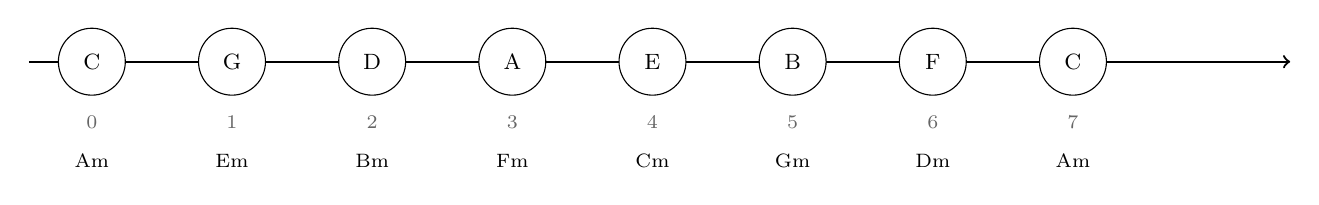
\begin{tikzpicture}[x=1.78cm,y=1cm,font=\footnotesize]
  \draw[->,thick] (-0.45,0) -- (8.55,0);
  \node[circle,draw,fill=white,minimum size=0.85cm,inner sep=0pt] (c0) at (0,0) {C};
  \node[circle,draw,fill=white,minimum size=0.85cm,inner sep=0pt] (c1) at (1,0) {G};
  \node[circle,draw,fill=white,minimum size=0.85cm,inner sep=0pt] (c2) at (2,0) {D};
  \node[circle,draw,fill=white,minimum size=0.85cm,inner sep=0pt] (c3) at (3,0) {A};
  \node[circle,draw,fill=white,minimum size=0.85cm,inner sep=0pt] (c4) at (4,0) {E};
  \node[circle,draw,fill=white,minimum size=0.85cm,inner sep=0pt] (c5) at (5,0) {B};
  \node[circle,draw,fill=white,minimum size=0.85cm,inner sep=0pt] (c6) at (6,0) {F\sharpsym};
  \node[circle,draw,fill=white,minimum size=0.85cm,inner sep=0pt] (c7) at (7,0) {C\sharpsym};
  \foreach \i/\sig in {0/0,1/1\sharpsym,2/2\sharpsym,3/3\sharpsym,4/4\sharpsym,5/5\sharpsym,6/6\sharpsym,7/7\sharpsym} {
    \node[below=16pt,font=\scriptsize,text=black!60] at (\i,0) {\sig};
  }
  \foreach \i/\mn in {0/{Am},1/{Em},2/{Bm},3/{F\sharpsym m},4/{C\sharpsym m},5/{G\sharpsym m},6/{D\sharpsym m},7/{A\sharpsym m}} {
    \node[below=30pt,font=\scriptsize] at (\i,0) {\mn};
  }
\end{tikzpicture}

\small Figure 4-2. The circle of fifths unrolled. Each step right raises the tonic by a perfect fifth and adds one sharp; below each circle is the key signature, then the relative minor. Going left adds flats: F major has one flat, B\flatsym{} major two, and so on.
\end{figure}

Major and minor keys with the same signature are relative keys. C major and A minor both have no accidentals; G major and E minor both have one sharp; F major and D minor both have one flat. The relative minor's tonic is a minor third below the major tonic (or a major sixth above it), for example A below C.

Do not confuse this with parallel major and minor: C major and C minor share a tonic but have different signatures, so they are parallel; C major and A minor share a signature but have different tonics, so they are relative.

\section{The pentatonic scale}

The pentatonic scale uses only five degrees and naturally avoids some semitone clashes. The most common major pentatonic takes degrees 1, 2, 3, 5, and 6 of the major scale, omitting 4 and 7:

\[
\mathrm{C4\ D4\ E4\ G4\ A4}.
\]

In the Chinese tradition this is the gong--shang--jue--zhi--yu system, corresponding to C, D, E, G, A; taking A as yu gives the A-yu mode with the same five pitches. The minor pentatonic takes 1, \(\flat\)3, 4, 5, and \(\flat\)7:

\[
\mathrm{A3\ C4\ D4\ E4\ G4}.
\]

The stability of the pentatonic scale comes from having no adjacent semitones: in the C major pentatonic every neighbouring pair is at least two semitones apart, so melodies rarely hit a sharp semitone clash. It is useful for quickly writing folk-flavoured lines, pop choruses, or riffs; when you need richer harmony, add the omitted 4 and 7 back.

\section{Common modes}

A mode can be understood as ``the same major scale with a different tonic.'' Using the seven notes of C major and taking C, D, E, F, G, A, B as tonic in turn gives seven modes. You can also rebuild each mode from its tonic with a semitone formula.

\begin{center}
\footnotesize
\renewcommand{\arraystretch}{1.12}
\setlength{\tabcolsep}{3pt}
\begin{longtable}{p{0.18\linewidth}p{0.34\linewidth}p{0.24\linewidth}p{0.15\linewidth}}
\toprule
Mode & Scale on C & Semitone formula & Character \\
\midrule
\endhead
Ionian & C D E F G A B & 2,2,1,2,2,2,1 & the major scale \\
Dorian & C D E\flatsym{} F G A B\flatsym & 2,1,2,2,2,1,2 & minor with natural sixth \\
Phrygian & C D\flatsym{} E\flatsym{} F G A\flatsym{} B\flatsym & 1,2,2,2,1,2,2 & flat second; heavy opening \\
Lydian & C D E F\sharpsym{} G A B & 2,2,2,1,2,2,1 & sharp fourth; bright, floating \\
Mixolydian & C D E F G A B\flatsym & 2,2,1,2,2,1,2 & major with flat seventh \\
Aeolian & C D E\flatsym{} F G A\flatsym{} B\flatsym & 2,2,1,2,2,1,2 & natural minor \\
Locrian & C D\flatsym{} E\flatsym{} F G\flatsym{} A\flatsym{} B\flatsym & 1,2,2,1,2,2,2 & flat second and flat fifth; least stable \\
\bottomrule
\end{longtable}

Table 4-2. The seven modes. The table writes them all on C for easy comparison; in practice the tonic can move and the formula stays the same.
\end{center}

A mode's flavour usually comes from one or two characteristic notes: Dorian's \(\sharp\)6 (a natural sixth, raised relative to natural minor), Phrygian's \(\flat\)2, Lydian's \(\sharp\)4, Mixolydian's \(\flat\)7, and Locrian's \(\flat\)2 and \(\flat\)5. When writing a melody, put the characteristic note where it can be heard, or the mode will not establish itself; changing the tonic without touching the characteristic note leaves the sound ambiguous.

\section{How to do it in Yeban}

\begin{enumerate}
  \item Open the piano roll (\texttt{P}/\texttt{F7}). Adjacent rows are semitones, so you can write a scale directly by row distance: for C major from the C4 row, place notes at +0, +2, +4, +5, +7, +9, +11, and +12, giving C4 D4 E4 F4 G4 A4 B4 C5.
  \item For A natural minor, start on the A3 row and place +0, +2, +3, +5, +7, +8, +10, +12; for A harmonic minor, raise the seventh degree G to G\sharpsym{} (move it up one row), then play both versions to compare.
  \item The \texttt{KEY / SCALE} readout in the top transport bar cycles through only three presets (C Minor (natural minor), D Dorian, F Major (major)), and clicking it changes the project's key-signature metadata. It does not automatically colour the roll rows by scale degree, and it does not offer arbitrary mode selection. For this chapter, trust the notes you place on the roll rather than treating that readout as a full scale tool.
  \item To hear relative keys, use the same white-key set (C D E F G A B). In the first version start on C and put the strong beat on C; in the second start on A and put the strong beat on A. The pitch material has not changed, but the tonic has, so the feel shifts from major to minor.
  \item For the pentatonic scale, keep only C4, D4, E4, G4, A4 in C major pentatonic and delete F4 and B4; for A minor pentatonic keep A3, C4, D4, E4, G4. Add the omitted notes back when you need denser harmony.
  \item Use A4 = 440 Hz as the reference for all pitch judgments; calibrate monitoring level and playback speed before judging a mode by ear.
\end{enumerate}

\screenshot{piano-roll-scale-ladder}{Scale ladder in the piano roll}{Scale ladder in the piano roll}

\textbf{Scope note:} Yeban currently has no dedicated panel that lays out a scale or labels scale degrees for a chosen mode. The top \texttt{KEY / SCALE} readout has only three presets and does not drive piano-roll colouring. The steps in this chapter rely on manual note placement plus row-distance checks, not on a scale-generation button that does not exist.

\section{Scales and modes in real songs}

\begin{itemize}
  \item \textbf{The Beatles, ``Let It Be''} (C major): Stays squarely inside the natural major scale with stepwise landings that anchor its comforting, steady mood.
  \item \textbf{Billie Eilish, ``bad guy''} (G minor): A spare minor bass riff with chromatic turns creates playful, dark modern pop tension without dense chords.
  \item \textbf{``Scarborough Fair''} (D Dorian): Keeps the raised sixth degree (B) inside a minor frame, yielding an archaic, bittersweet colour that is neither plain sad nor bright.
\end{itemize}

\section{Exercises}


\begin{exercise}
\begin{enumerate}
  \item Write the seven degrees of C major and the semitone count between adjacent degrees; how many semitones separate B4 and C5?\\
  \emph{Answer:} C D E F G A B; \(2,2,1,2,2,2,1\); B4--C5 is one semitone.

  \item Write the notes of A natural minor and its relative major; raising the seventh gives which minor, and which note is raised?\\
  \emph{Answer:} A B C D E F G; relative major C major; raising G gives A harmonic minor.

  \item A key signature with three sharps belongs to which relative pair, and what are the two tonics?\\
  \emph{Answer:} A major (A) and F\sharpsym{} minor (F\sharpsym); the sharps are F\sharpsym, C\sharpsym, G\sharpsym.

  \item Which notes belong to the C major pentatonic, and which two degrees are omitted? What about A minor pentatonic?\\
  \emph{Answer:} C D E G A; degrees 4 (F) and 7 (B) are omitted; A minor pentatonic is A C D E G.

  \item In Yeban, write the seven notes of D Dorian starting on D4, and explain its relation to C major.\\
  \emph{Hint:} D Dorian uses the notes of C major with D as tonic: D E F G A B C. On the roll, start at the D4 row and place notes at +0, +2, +3, +5, +7, +9, +10 rows; the final C is at C5, ten semitones above D4.\\
  \emph{Answer:} D E F G A B C; the note set is the same as C major but the tonic is D, and the natural sixth B is the Dorian marker.
\end{enumerate}
\end{exercise}

\section{Help topic map}

\begin{center}
\footnotesize
\setlength{\tabcolsep}{3pt}
\begin{longtable}{p{0.34\linewidth}p{0.45\linewidth}p{0.15\linewidth}}
\toprule
Section & In-app help anchor & Note \\
\midrule
\endhead
Scales and degrees & \texttt{music-theory-scale-degrees} & concept \\
Major scale & \texttt{music-theory-major-scale} & Figure 4-1 \\
The three minor forms & \texttt{music-theory-minor-scales} & Table 4-1 \\
Key signatures and the circle & \texttt{music-theory-key-signature-circle} & Figure 4-2 \\
Relative keys & \texttt{music-theory-relative-keys} & concept \\
Pentatonic scale & \texttt{music-theory-pentatonic} & formula \\
Common modes & \texttt{music-theory-modes} & Table 4-2 \\
How to do it in Yeban & \texttt{music-theory-piano-roll-scales} & procedure \\
Exercises & \texttt{music-theory-ch4-practice} & answers above \\
\bottomrule
\end{longtable}
\end{center}

\section*{Further reading}
\begin{itemize}
  \item \textbf{Open Music Theory, “Scales and scale degrees.”} \url{https://openmusictheory.github.io/scales.html} — builds scales from scale degrees and tonic, then connects modes and key signatures.
  \item \textbf{YouTube, “Modes and Scales” playlist.} \url{https://www.youtube.com/playlist?list=PLlx2eo2tD6KoGvA_q0DFrYeLuwklZEy0O} — uses real songs to compare the seven modes by sound instead of memorized patterns.
\end{itemize}

